\usepackage{fixltx2e}[2006/03/24]
\usepackage[utf8]{inputenc}
\usepackage[T1]{fontenc}
\usepackage{textcomp}
\usepackage{lmodern}
\usepackage[british,french]{babel}
\usepackage[babel]{microtype}
\usepackage{xspace} % load after babel
\usepackage{graphicx}
\usepackage[center,tight]{subfigure}
\usepackage{hyperref}
%\usepackage{cite}
%\usepackage{array}
%\usepackage{booktabs}
%\usepackage{varioref}

\usepackage{bm}
\usepackage{mathtools}
\usepackage[strict, separate-uncertainty, output-decimal-marker={,}]{siunitx}


\AtBeginSection[] {
  \begin{frame}<beamer>{Plan}
    \tableofcontents[currentsection]
  \end{frame}
}
\mode<article>{
  \newenvironment{eq}{\begin{equation}}{\end{equation}}
  \usepackage{fancyhdr}
  \pagestyle{fancy}
  \renewcommand{\headrulewidth}{0pt}\fancyhead{} % Remove header
}
\mode<presentation>{
  \newenvironment{eq}{\begin{equation*}}{\end{equation*}}
}


\newcommand{\lAB}{\texorpdfstring{\ensuremath{l\alpha \beta}}{lαβ}\xspace}
\newcommand{\code}[1]{\textsf{#1}}

\title{Transfert de couleurs entre images}
\subtitle{Projet C++ en Magistère 2}
\author{Yann Leprince}

\begin{document}
\mode<presentation>{\microtypesetup{expansion=false}}
\setbeamertemplate{frametitle}{}
\lfoot{\footnotesize \href{mailto:yann.leprince@u-psud.fr}
                     {Yann Leprince <\textsf{yann.leprince@u-psud.fr}>}}
\rfoot{\footnotesize \today}


\frame{\maketitle}

\begin{frame}<handout>{Plan}
  \tableofcontents
\end{frame}


\begin{abstract}
Pour ce projet vous devrez implémenter une méthode de traitement d'image,
consistant à transférer les couleurs d'une image vers une autre.

Un exemple est présenté en figure \ref{fig:exemple_transfert}. L'image source
est ici un rendu informatique d'une scène virtuelle, l'image cible une
photographie. L'image résultat représente la scène de l'image source, mais a
acquis la dominante colorée de l'image cible.
\end{abstract}

\vspace{1.5cm}

\begin{figure}[h!]
  \centering
  \subfigure[Source]{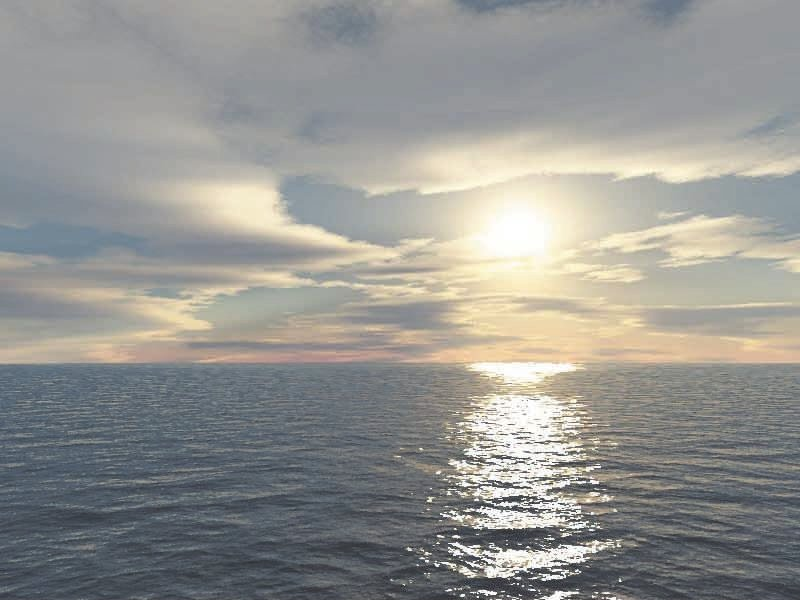
\includegraphics[width=5cm]{source}}
  \subfigure[Cible]{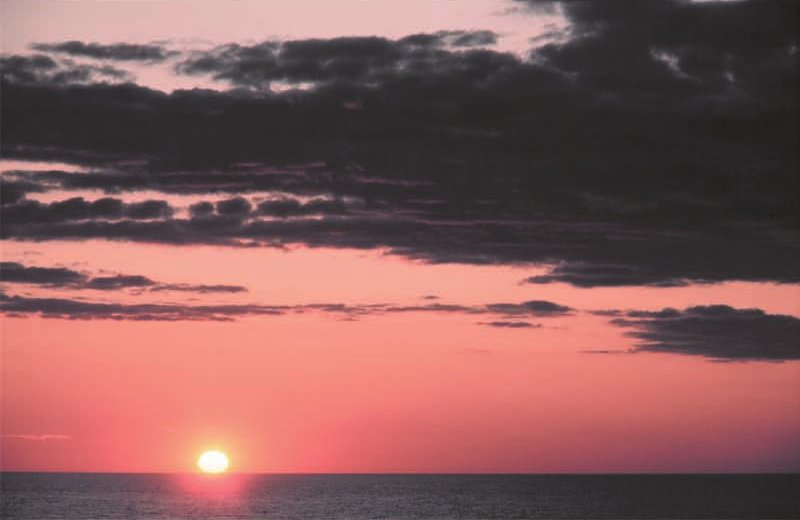
\includegraphics[width=5cm]{target}}
  \subfigure[Résultat]{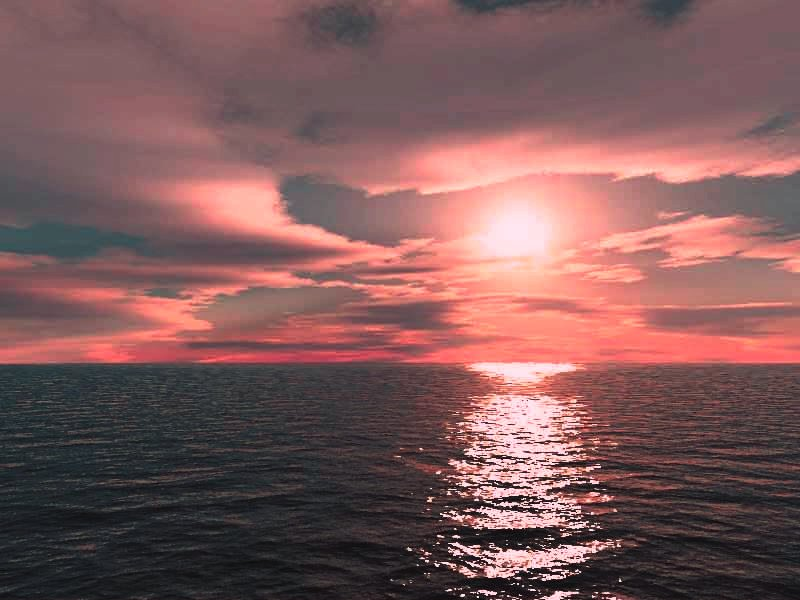
\includegraphics[width=5cm]{srcsourcetgttarget}}
  \caption{Exemple de transfert de couleurs}
  \label{fig:exemple_transfert}
\end{figure}

\clearpage

\section*{Introduction au transfert de couleurs}
\label{sec:intro_transfert}

\begin{frame}<presentation>{Transfert de couleurs~?}
  \begin{columns}
    \column{6cm}
    \centering
    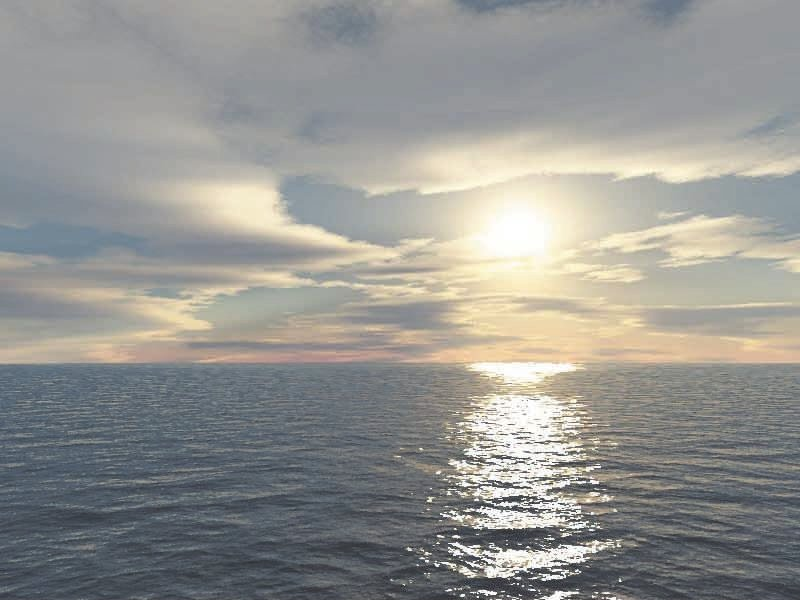
\includegraphics[width=4cm]{source}

    Source

    \vspace{2ex}
    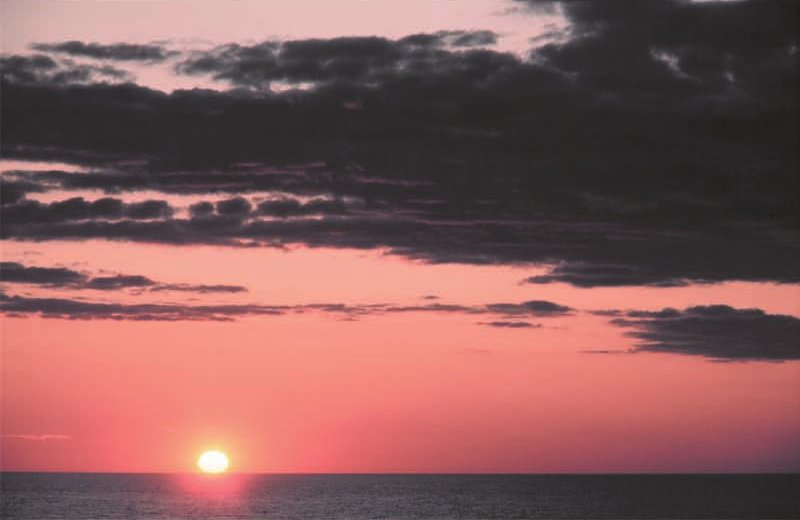
\includegraphics[width=4cm]{target}

    Cible

    \pause

    \column{6cm}
    \centering
    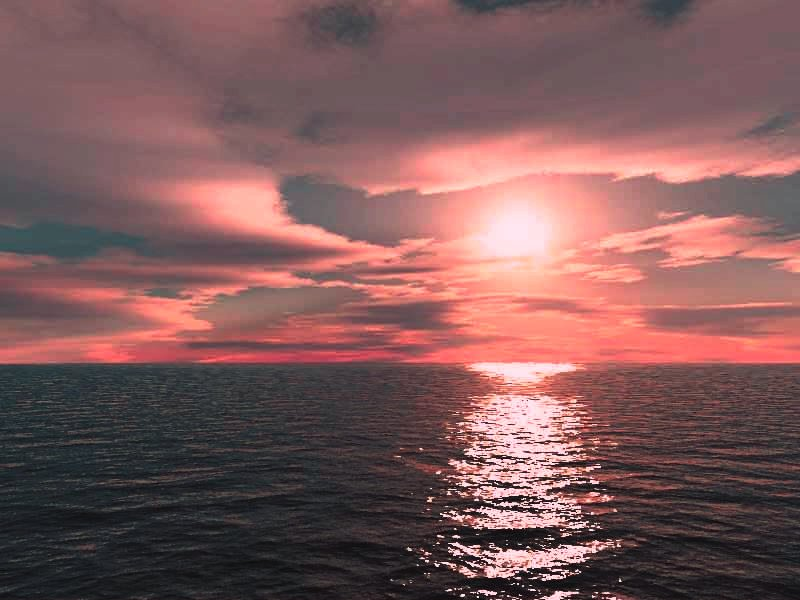
\includegraphics[width=6cm]{srcsourcetgttarget}

    Résultat
  \end{columns}
\end{frame}

Partant de deux images appelées respectivement \emph{source} et \emph{cible,}
le transfert de couleurs consiste à calculer une troisième image, appelée
\emph{résultat,} qui est une version de l'image source modifiée pour que ses
caractéristiques colorimétriques s'approchent de celles de l'image cible. En
d'autres termes, l'image résultat représente la scène de l'image source, mais
ses couleurs ressemblent à celle de l'image cible. La méthode décrite ici
provient d'un article~\cite{reinhard01:color_transfer} que vous pouvez
consulter pour en savoir plus sur son fonctionnement.


\section{Méthode à implémenter}
\label{sec:descr_meth}

\subsection{Rappel sur les images}
\label{sec:intro_image}

\begin{frame}<presentation>{L'image, une grille de pixels}
  L'image est une grille dont chaque pixel contient\\
  une information de couleur.

  \pause

  \begin{itemize}
  \item Trois composantes car trois types de capteurs rétiniens
  \item Habituellement composantes RVB car les écrans et les capteurs
    fonctionnent ainsi
    \begin{itemize}
    \item Rouge
    \item Vert
    \item Bleu
    \end{itemize}

  \pause

  \item Exemples
    \begin{itemize}
    \item $(0; 0; 0)$ = noir
    \item $(1; 0; 0)$ = rouge vif
    \item $(1; 1; 1)$ = blanc
    \end{itemize}

    \pause

  \item Il existe d'autres \alert{espaces colorimétriques}
  \end{itemize}
\end{frame}

Les images que vous manipulerez dans ce projet sont des images
bidimensionnelles en couleurs. Elles sont constituées de pixels disposés sur
une grille carrée, repérés par une abscisse et une ordonnée. Chaque pixel
contient une couleur sous la forme d'un vecteur à trois composantes.
L'interprétation de ces composantes dépend de l'\emph{espace colorimétrique}
dans lequel est exprimée la couleur. Vous utiliserez deux espaces
colorimétriques distincts: l'espace RVB pour le stockage des images, et
l'espace \lAB plus adapté au transfert de couleurs.

L'espace colorimétrique RVB représente une couleur comme un mélange additif de
lumières rouge, verte, et bleue. Ainsi le vecteur $(1; 0; 0)$ dans cet espace
représente un rouge pur, le vecteur $(1; 1; 0)$ un jaune vif (rouge + vert en
synthèse additive), le vecteur $(\num{0.5}; \num{0.5}; \num{0.5})$ un gris
moyen. Chaque composante est comprise dans l'intervalle $[0; 1]$. Cet espace
colorimétrique est largement utilisé pour la capture, le stockage, et la
représentation des images numériques car il correspond à la technique utilisée
par les capteurs et les écrans.

L'espace RVB, en revanche, ne rend pas bien compte de la perception des
couleurs par l'œil humain. Pour produire un résultat visuellement satisfaisant,
le transfert de couleurs doit se faire dans un espace mieux adapté.


\subsection{Espace colorimétrique \lAB}
\label{sec:espace_lab}

\begin{frame}<presentation>{Espace colorimétrique \lAB}
  \begin{itemize}
  \item Issu de recherches sur la perception humaine
  \item Un canal achromatique $l$: luminosité
  \item Deux canaux chromatiques
    \begin{itemize}
    \item $\alpha$: opposition bleu--jaune
    \item $\beta$: opposition vert--rouge
    \end{itemize}
  \item Composantes décorrélées pour les images naturelles
  \end{itemize}
\end{frame}

L'espace colorimétrique \lAB utilise, pour représenter une couleur, des
composantes notées respectivement $l$, $\alpha$, et $\beta$. Cet espace a été
défini à partir de recherches sur la perception humaine des couleurs. Ainsi, la
distance euclidienne entre deux points de cet espace tridimensionnel est
approximativement proportionnelle à la différence perceptuelle entre les deux
couleurs correspondantes. Deux couleurs perçues comme similaires seront proches
dans l'espace tridimensionnel \lAB, deux couleurs perçues comme différentes y
seront éloignées.

L'espace \lAB présente un autre avantage: son canal $l$ représente la sensation
de luminance, c'est-à-dire la quantité d'énergie contenue dans une couleur
donnée, et les canaux $\alpha$ et $\beta$ représentent la chrominance,
c'est-à-dire la \og{}teinte\fg{}. Ces trois canaux sont aussi décorrélés que
possible pour des images naturelles, ce qui rend pertinente l'application de
statistiques univariées dans chaque canal indépendamment des autres
(§~\ref{sec:transf_stat}).


\subsection{Changement d'espace colorimétrique}
\label{sec:changement_espace}

Le passage d'un espace colorimétrique à un autre correspond à un changement de
variables dans un espace tridimensionnel. Dans le cas du passage de RVB à \lAB,
ce changement est non linéaire et se définit en deux étapes, en passant par les
variables intermédiaires $L$, $M$, et $S$.

\begin{frame}{Changement d'espace colorimétrique}

  \only<presentation>{On utilise l'espace intermédiaire $LMS$.}

  \begin{eq}
  \begin{pmatrix}
    L \\ M \\ S
  \end{pmatrix}
  =
  \begin{pmatrix*}[S]
    0.3811 & 0.5783 & 0.0402 \\
    0.1967 & 0.7244 & 0.0782 \\
    0.0241 & 0.1288 & 0.8444
  \end{pmatrix*}
  \begin{pmatrix}
    R \\ V \\ B
  \end{pmatrix}
  \label{eq:rvb2lms}
  \end{eq}

  \begin{eq}
  \begin{pmatrix}
    l \\ \alpha \\ \beta
  \end{pmatrix}
  =
  \begin{pmatrix}
    1 / \sqrt{3} & 0 & 0 \\
    0 & 1 / \sqrt{6} & 0 \\
    0 & 0 & 1 / \sqrt{2}
  \end{pmatrix}
  \begin{pmatrix}
    1 & 1 & 1 \\
    1 & 1 & -2 \\
    1 & -1 & 0
  \end{pmatrix}
  \begin{pmatrix}
    \ln L \\ \ln M \\ \ln S
  \end{pmatrix}
  \label{eq:lms2lab}
  \end{eq}
\end{frame}


\subsection{Transfert de statistiques}
\label{sec:transf_stat}

Une fois dans l'espace colorimétrique \lAB, le transfert de couleurs consiste à
calculer une transformation affine pour chaque canal de l'image source, de
façon à rendre les moments statistiques d'ordre un et deux (moyenne et
écart-type) égaux à ceux de l'image cible. Cette transformation est ensuite
appliquée à tous les pixels de l'image source.

Pour connaître cette transformation il est nécessaire de calculer la moyenne et
l'écart-type de chaque canal, pour l'image source et pour l'image cible. Ainsi
pour le canal $l$, on prend en compte tous les pixels de l'image source pour
calculer la moyenne $\bar{l}_s$ et l'écart-type $\sigma^l_s$. En faisant de
même dans l'image cible on calcule la moyenne $\bar{l}_c$ et l'écart-type
$\sigma^l_c$. Le calcul est identique pour les statistiques des canaux $\alpha$
et $\beta$: $\bar{\alpha}_s$ et $\sigma^\alpha_s$, $\bar{\alpha}_c$ et
$\sigma^\alpha_c$, $\bar{\beta}_s$ et $\sigma^\beta_s$, $\bar{\beta}_c$ et
$\sigma^\beta_c$.

Une fois connues les valeurs de ces moments statistiques, on peut appliquer les
formules \ref{eq:transf_stat_l}, \ref{eq:transf_stat_alpha}, et
\ref{eq:transf_stat_beta} pour obtenir les nouvelles valeurs $(l_r, \alpha_r,
\beta_r)$ de chaque pixel de l'image résultat, en fonction des valeurs $(l,
\alpha, \beta)$ du pixel correspondant dans l'image source.

\pagebreak

\begin{frame}{Transfert de statistiques}
  \only<presentation>{
    \begin{itemize}
    \item Transfert de moyenne et d'écart-type
    \item Indépendamment dans chaque canal
    \end{itemize}
  }
  \begin{align}
    l_r &= \frac{\sigma^l_c}{\sigma^l_s}(l-\bar{l}_s) + \bar{l}_c
    \label{eq:transf_stat_l}
    \\
    \alpha_r &=
    \frac{\sigma^{\alpha}_c}{\sigma^{\alpha}_s}(\alpha-\bar{\alpha}_s)
    + \bar{\alpha}_c
    \label{eq:transf_stat_alpha}
    \\
    \beta_r &=
    \frac{\sigma^{\beta}_c}{\sigma^{\beta}_s}(\beta-\bar{\beta}_s)
    + \bar{\beta}_c
    \label{eq:transf_stat_beta}
  \end{align}
\end{frame}

On vérifie aisément qu'après cette transformation la distribution des valeurs
de l'image résultat est identique à celle de l'image cible dans chaque canal,
au sens des moments d'ordre un et deux.


\subsection{Retour dans l'espace RVB}
\label{sec:retour_rvb}

Une fois l'image résultat calculée, il reste à repasser dans l'espace RVB pour
pouvoir la sauvegarder et la visualiser. Pour cela on utilise la transformation
inverse de celle décrite précédemment.

\begin{frame}{Retour dans l'espace colorimétrique initial}
  \begin{eq}
  \begin{pmatrix}
    \bm{L} \\ \bm{M} \\ \bm{S}
  \end{pmatrix}
  =
  \begin{pmatrix}
    1 & 1 & 1 \\
    1 & 1 & -1 \\
    1 & -2 & 0
  \end{pmatrix}
  \begin{pmatrix}
    1 / \sqrt{3} & 0 & 0 \\
    0 & 1 / \sqrt{6} & 0 \\
    0 & 0 & 1 / \sqrt{2}
  \end{pmatrix}
  \begin{pmatrix}
    l \\ \alpha \\ \beta
  \end{pmatrix}
  \label{eq:lab2lms}
  \end{eq}

  \begin{eq}
  \begin{pmatrix}
    R \\ V \\ B
  \end{pmatrix}
  =
  \begin{pmatrix*}[S]
    4.4679 & -3.5873 & 0.1193 \\
    -1.2186 & 2.3809 & -0.1624 \\
    0.0497 & -0.2439 & 1.2045
  \end{pmatrix*}
  \begin{pmatrix}
    \exp \bm{L} \\ \exp \bm{M} \\ \exp \bm{S}
  \end{pmatrix}
  \label{eq:lms2rvb}
  \end{eq}
\end{frame}

\subsection<presentation>{Transfert global de statistiques}
\label{sec:res_trans_global}

\begin{frame}<presentation>{Exemple favorable}
  \begin{columns}
    \column{6cm}
    \centering
    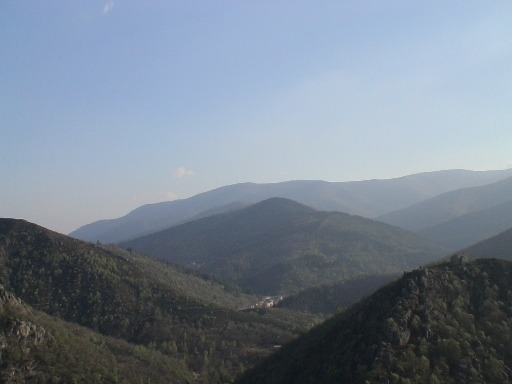
\includegraphics[width=4cm]{DSC04659}

    Source

%    \column{4cm}
%    \centering
    \vspace{2ex}
    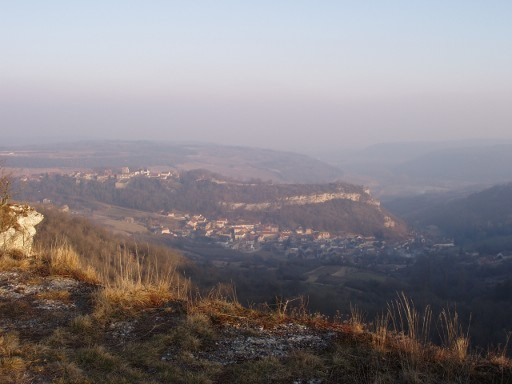
\includegraphics[width=4cm]{P2130173}

    Cible

    \column{6cm}
    \centering
    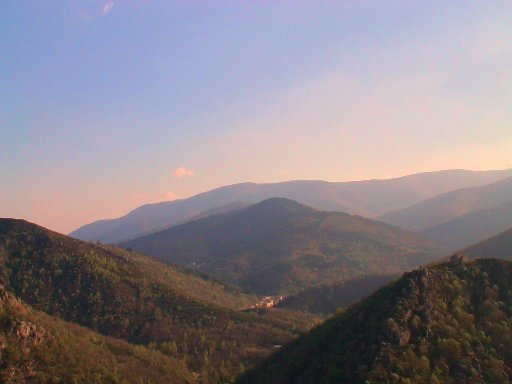
\includegraphics[width=6cm]{srcDSC04659tgtP2130173}

    Résultat
  \end{columns}
\end{frame}

\begin{frame}<presentation>{Changement d'éclairage, de balance des blancs}
  \begin{columns}
    \column{6cm}
    \centering
    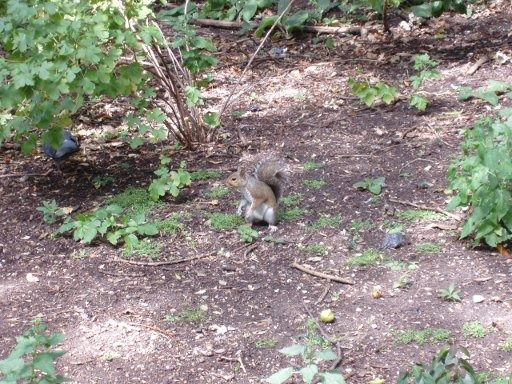
\includegraphics[width=4cm]{p7250101}

    Source

%    \column{4cm}
%    \centering
    \vspace{2ex}
    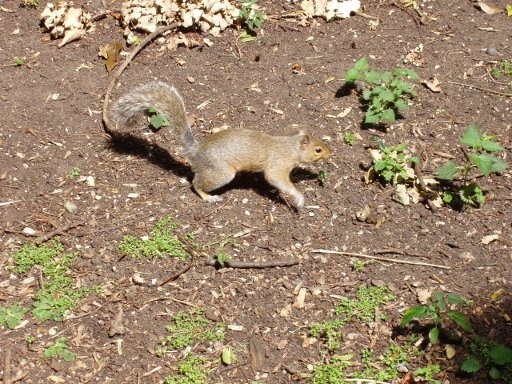
\includegraphics[width=4cm]{p7250102}

    Cible

    \column{6cm}
    \centering
    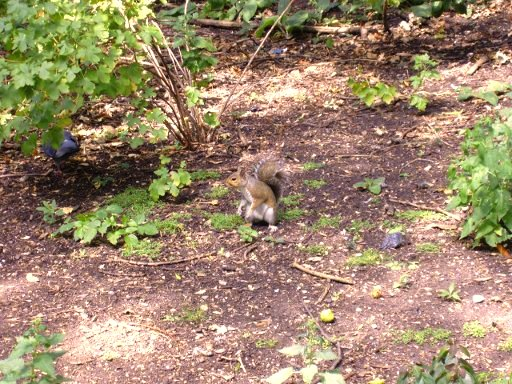
\includegraphics[width=6cm]{srcp7250101tgtp7250102}

    Résultat
  \end{columns}
\end{frame}

\begin{frame}<presentation>{Exemple défavorable}
  \begin{columns}
    \column{6cm}
    \centering
    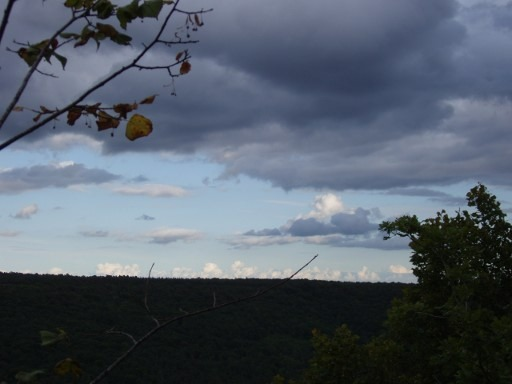
\includegraphics[width=4cm]{P8170066}

    Source

%    \column{4cm}
%    \centering
    \vspace{2ex}
    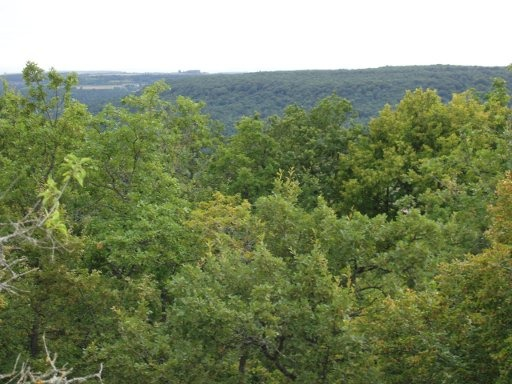
\includegraphics[width=4cm]{P8170082}

    Cible

    \column{6cm}
    \centering
    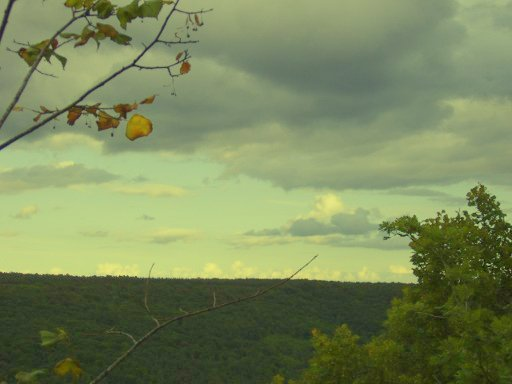
\includegraphics[width=6cm]{srcP8170066tgtP8170082}

    Résultat
  \end{columns}
\end{frame}


\section{Récapitulatif du travail à effectuer}
\label{sec:recapitulatif}

Vous implémenterez la méthode décrite (§~\ref{sec:descr_meth}), en vous aidant
des quelques repères d'implémentation fournis (§~\ref{sec:implementation}).
Vous déciderez vous-même de la structure votre programme (liste des classes,
notamment); en accord avec votre encadrant qui pourra vous guider en cas de
difficulté.

En résumé, votre programme devra effectuer, dans l'ordre, ces opérations:

\begin{frame}{Récapitulatif du travail à effectuer}
  \begin{enumerate}
  \item Chargement des images RVB source et cible (fonction fournie)
  \item Conversion $\text{RVB} \to \lAB$
  \item Calcul des statistiques (moyenne, écart-type)
  \item Transformation linéaire de chaque pixel de l'image source
  \item Conversion du résultat $\lAB \to \text{RVB}$
  \item Écriture du résultat (fonction fournie)
  \end{enumerate}

  \only<presentation>{
    \vspace{5mm}

    {\footnotesize
      \begin{thebibliography}{1}

      \bibitem{reinhard01:color_transfer}
        E.~Reinhard, M.~Ashikhmin, B.~Gooch, et P.~Shirley.
        \newblock {\em Color transfer between images}.
        \newblock {\em IEEE Computer Graphics and Applications}, 21(5): 34--41,
        septembre 2001.

      \end{thebibliography}
    }
  }
\end{frame}

\mode<article>{ % Whole section in article only
\section{Aspects d'implémentation}
\label{sec:implementation}

Les fichiers nécessaires à la réalisation du projet vous seront fournis par vos
encadrants.

Les images au format RVB sont habituellement stockées avec 24~bits par pixel.
Chaque canal est codé sous la forme d'un entier non signé de 8~bits, dans
l'intervalle $[0; 255]$. Les changements d'espace colorimétriques décrits
ci-dessus (§~\ref{sec:changement_espace} et §~\ref{sec:retour_rvb}) s'entendent
pour des valeurs comprises entre 0 et 1, il faut donc effectuer une conversion
au chargement, et la conversion inverse à la sauvegarde.

Une classe vous est fournie pour charger et sauvegarder des images stockées au
format BMP \og{}\emph{Windows bitmap}\fg{} à 24~bits par pixel non compressées.
Seules les images dans ce format peuvent être lues, voir
l'annexe~\ref{sec:conversion_bmp24} pour la conversion depuis un autre format.
Cette classe est déclarée dans le fichier d'en-tête \code{bmp\_io.hh} et
définie dans le fichier \code{bmp\_io.cc}. Pour l'utiliser, vous devez donc
inclure \code{bmp\_io.hh}, et compiler et lier \code{bmp\_io.cc} parmi vos
propres fichiers compilés.

La documentation de la classe \code{Bmp24} se trouve dans les commentaires du
fichier \code{bmp\_io.hh}. Vous pouvez vous aider de l'exemple fourni dans le
fichier \code{bmp\_demo.cc}. Pour le compiler, faites \code{g++ -o bmp\_demo
bmp\_io.cc bmp\_demo.cc}.


} % End of whole section in article only

\section{Bonus: transfert de couleurs par zone}
\label{sec:trans_par_zone}

\begin{quote}
Attention, le travail décrit dans cette partie est considéré comme
un \textbf{bonus}. Commencez-le uniquement si vous estimez avoir implémenté de
votre mieux la partie obligatoire du sujet. Une implémentation propre de
celle-ci sera toujours préférée à une implémentation complète mais bâclée.
\end{quote}

L'article \cite{reinhard01:color_transfer} qui décrit la méthode que vous avez
implémentée en décrit également une variante plus sophistiquée, qui permet des
transferts de couleurs plus complexes. Le principe est de définir des zones
appairées dans les images source et cible, et de calculer une transformation de
l'espace \lAB indépendemment pour chaque paire. On calcule ensuite une image
résultat pour chacune de ces transformations. Ces multiples résultats sont
mélangés en utilisant des facteurs de pondération
$f^{(i)} \propto \frac{1}{d_{(i)}}$ calculés pour chaque pixel en fonction de
sa distance colorimétrique $d_{(i)}$ aux statistiques de chaque zone source
$(i)$, selon l'équation \ref{eq:dist_classe}.

\begin{eq}
d^2_{(i)} = \left( \frac{l - \bar{l}_{(i)}}{\sigma_l^{(i)}} \right)^2
+ \left( \frac{\alpha - \bar{\alpha}_{(i)}}{\sigma_{\alpha}^{(i)}} \right)^2
+ \left( \frac{\beta - \bar{\beta}_{(i)}}{\sigma_{\beta}^{(i)}} \right)^2
\label{eq:dist_classe}
\end{eq}


\begin{frame}<presentation>{Exemple défavorable}
  \begin{columns}
    \column{4cm}
    \centering
    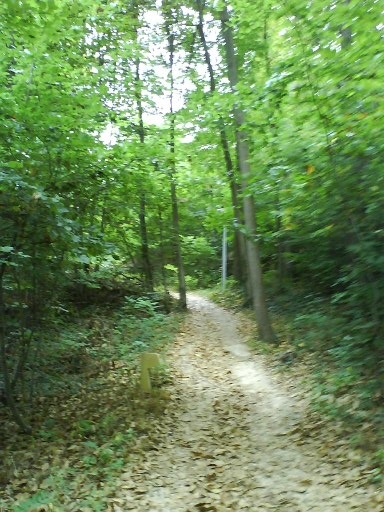
\includegraphics[width=4cm]{DSC00025}

    Source

    \column{4cm}
    \centering
    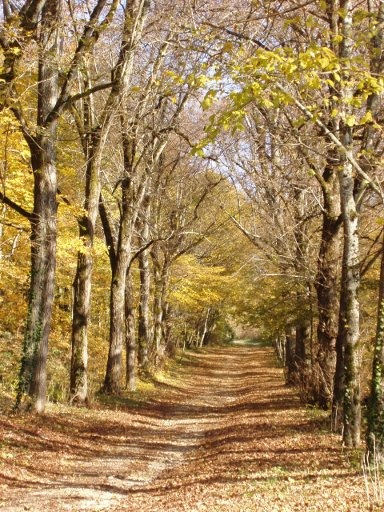
\includegraphics[width=4cm]{PB020097}

    Cible

    \column{4cm}
    \centering
    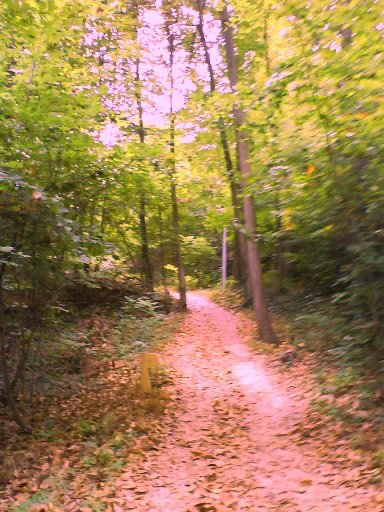
\includegraphics[width=4cm]{srcDSC00025tgtPB020097}

    Résultat
  \end{columns}
\end{frame}

\begin{frame}<presentation>{Sélection de zones}
  \begin{columns}
    \column{6cm}
    \centering
    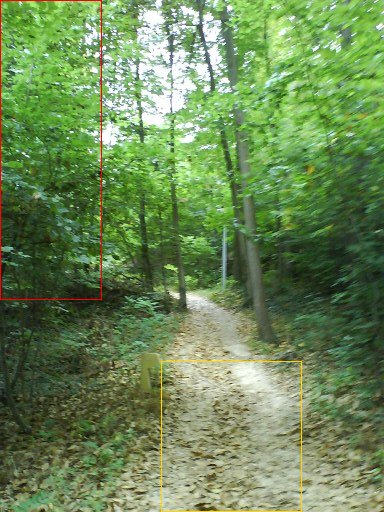
\includegraphics[width=4cm]{drawsrc}

    Source

    \column{6cm}
    \centering
    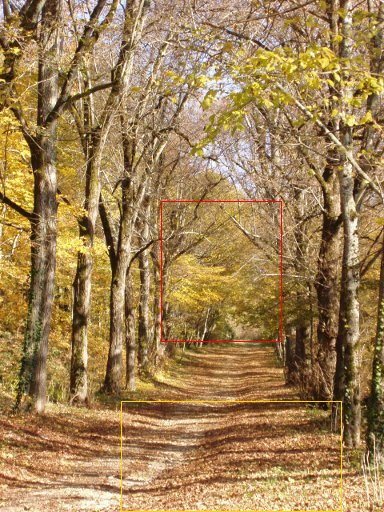
\includegraphics[width=4cm]{drawtgt}

    Cible
  \end{columns}
\end{frame}

\begin{frame}<presentation>{Transfert des statistiques partielles}
  \begin{columns}
    \column{6cm}
    \centering
    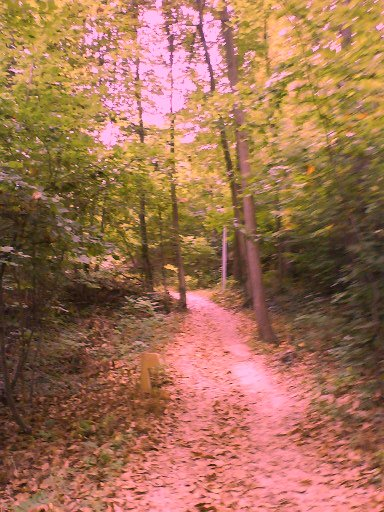
\includegraphics[width=4cm]{dst1}

    Transformation 1 \\ (feuilles)

    \column{6cm}
    \centering
    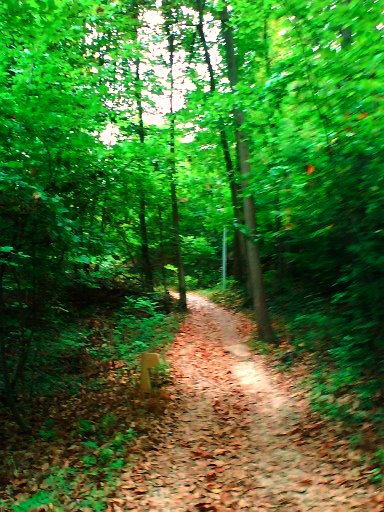
\includegraphics[width=4cm]{dst2}

    Transformation 2 \\ (chemin)
  \end{columns}
\end{frame}

\begin{frame}<presentation>{Fusion des images obtenues}
  \begin{columns}
    \column{6cm}
    Pour chaque pixel:

    \begin{multline*}
    d^2_{(i)} = \left( \frac{l - \bar{l}_{(i)}}{\sigma_l^{(i)}} \right)^2
    + \left( \frac{\alpha - \bar{\alpha}_{(i)}}{\sigma_{\alpha}^{(i)}} \right)^2 \\
    + \left( \frac{\beta - \bar{\beta}_{(i)}}{\sigma_{\beta}^{(i)}} \right)^2
    \end{multline*}

    \begin{eq}
    f^{(i)} \propto \frac{1}{d_{(i)}}
    \end{eq}

    \column{6cm}
    \centering
    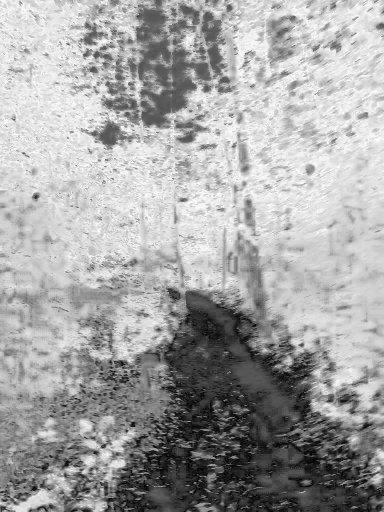
\includegraphics[width=4cm]{factors}

    Carte des facteurs de mélange
  \end{columns}
\end{frame}


Reportez-vous à l'article \cite{reinhard01:color_transfer} pour connaître les
détails de cette méthode améliorée, et n'hésitez pas à contacter votre
encadrant si vous avez besoin de précisions.


\begin{frame}<presentation>{Comparasion transfert global -- par zone}
  \begin{columns}
    \column{6cm}
    \centering
    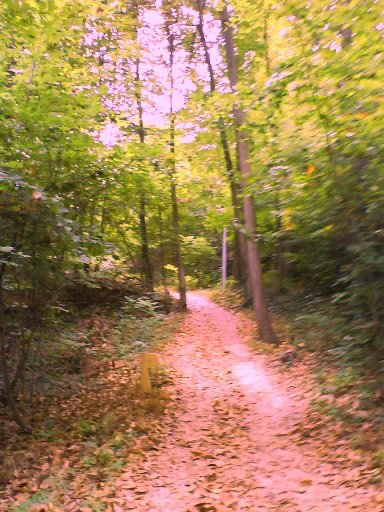
\includegraphics[width=4cm]{srcDSC00025tgtPB020097}

    Transfert global

    \column{6cm}
    \centering
    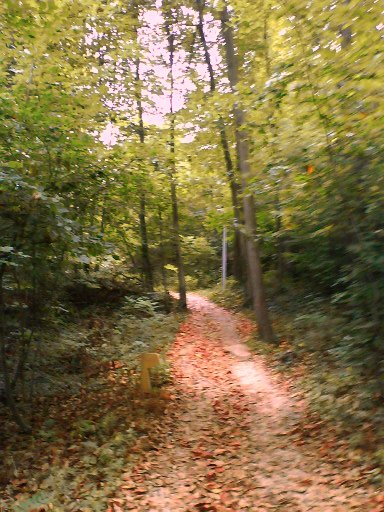
\includegraphics[width=4cm]{res}

    Transfert par zone et fusion
  \end{columns}
\end{frame}




\appendix

\begin{frame}<presentation>{Transfert de statistiques dans l'espace RVB}
  \begin{columns}
    \column{6cm}
    \centering
    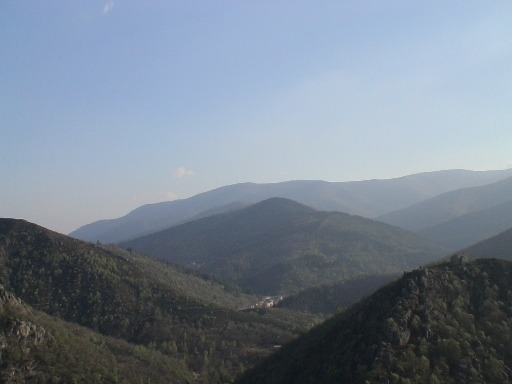
\includegraphics[width=4cm]{DSC04659}

    Source

%    \column{4cm}
%    \centering
    \vspace{2ex}
    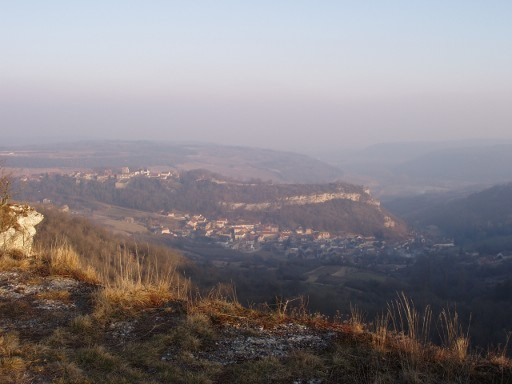
\includegraphics[width=4cm]{P2130173}

    Cible

    \column{6cm}
    \centering
    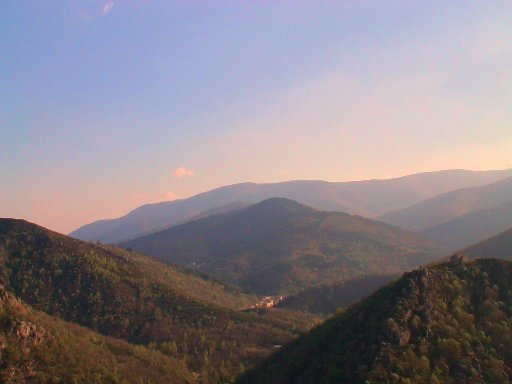
\includegraphics[width=4cm]{srcDSC04659tgtP2130173}

    Résultat \lAB

    \vspace{2ex}
    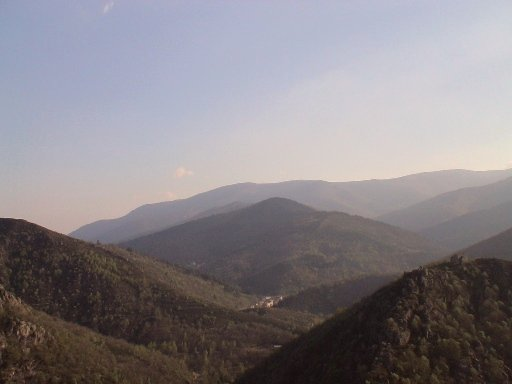
\includegraphics[width=4cm]{RGBsrcDSC04659tgtP2130173}

    Résultat RVB
  \end{columns}
\end{frame}


\section<article>{Convertir une image en BMP 24~bits}
\label{sec:conversion_bmp24}

Vous pouvez convertir une image au format BMP 24~bits en utilisant GIMP, un
éditeur d'images libre téléchargeable
sur \href{http://www.gimp.org/}{gimp.org}:

\begin{enumerate}
\item Chargez l'image souhaitée avec Fichier\slash{}Ouvrir.
\item Vérifiez que l'image est en mode RVB avec Image\slash{}Mode\slash{}RVB.
\item Enregistrez l'image avec Fichier\slash{}Enregistrer sous. Sélectionnez le
  format BMP (extension de nom de fichier \code{.bmp}). Validez.
\item Dans l'écran qui apparaît, sélectionnez \og{}Options avancées\fg{}
puis \og{}R8 G8 B8\fg{} sous \og{}24~bits\fg{} (voir figure
\ref{fig:capture_gimp_bmp}).
\end{enumerate}

\begin{figure}[h]
  \centering
  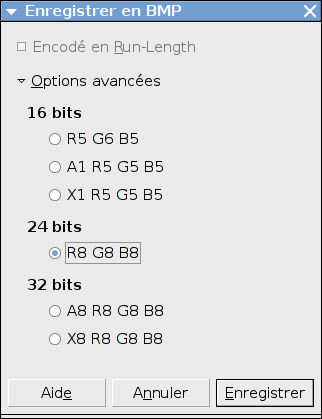
\includegraphics[width=5cm]{capture-gimp-bmp}
  \caption{Enregistrer une image BMP 24~bits avec GIMP.}
  \label{fig:capture_gimp_bmp}
\end{figure}


\mode<article>{
  \begin{thebibliography}{1}

  \bibitem{reinhard01:color_transfer}
    E.~Reinhard, M.~Ashikhmin, B.~Gooch, et P.~Shirley.
    \newblock {\em Color transfer between images}.
    \newblock {\em IEEE Computer Graphics and Applications}, 21(5): 34--41,
    septembre 2001.
    \newblock Copie électronique disponible parmi les fichiers fournis.

  \end{thebibliography}
}

\end{document}
